\section{Results}
\label{sec:results}

\para{Behavioral individuality is measurable.}
\Tabref{tab:individuality} shows that homogeneous prompt variants do not qualify as distinct individuals by our behavioral criterion. Their individuality ratio is 0.9294, because between-agent distance (0.0625) is smaller than within-agent variance (0.0672). Role-diverse variants cross the threshold with an individuality ratio of 1.1873. This gives a concrete operational answer to the population question: separate sessions count as separate individuals only when their outputs diverge more than sampling noise alone would predict.

\begin{table}[t]
\centering
\caption{Behavioral individuality assay for the $P{=}4$ homogeneous and role-diverse populations. An individuality ratio above 1 means between-agent differences exceed within-agent stochastic variance.}
\label{tab:individuality}
\begin{tabular}{@{}lccc@{}}
\toprule
Condition & Within distance & Between distance & Individuality ratio \\
\midrule
Homogeneous $P{=}4$ assay & 0.0672 & 0.0625 & 0.9294 \\
Role-diverse $P{=}4$ assay & \textbf{0.0613} & \textbf{0.0728} & \textbf{1.1873} \\
\bottomrule
\end{tabular}
\end{table}


\para{There is no clean minimum viable population threshold.}
\Tabref{tab:final_results} compares the final generation across all six conditions. If a simple threshold existed, we would expect larger populations to dominate smaller ones. We do not observe that pattern. The best final condition is \textsc{P1-Homogeneous-Accumulation} with a collapse score of $-0.0072$, while the worst is \textsc{P4-Role-Diverse-Accumulation} with a collapse score of $0.3147$. Grouping by nominal population size yields mean final collapse scores of 0.0966 for $P{=}1$, 0.2056 for $P{=}2$, and 0.1858 for $P{=}4$, which again does not support a monotonic threshold.

\begin{table*}[t]
\centering
\resizebox{\textwidth}{!}{%
\begin{tabular}{@{}lcccc@{}}
\toprule
Condition & Final collapse score $\downarrow$ & Final truth rate $\uparrow$ & Final distinct-2 $\uparrow$ & Final token entropy $\uparrow$ \\
\midrule
\textsc{P1-Homogeneous-Accumulation} & \textbf{-0.0072} & 0.7500 & 0.9095 & 8.7962 \\
\textsc{P4-Homogeneous-Replacement} & 0.0190 & \textbf{0.8333} & 0.9041 & 8.8324 \\
\textsc{P1-Homogeneous-Replacement} & 0.2003 & 0.6667 & \textbf{0.9394} & \textbf{8.9622} \\
\textsc{P2-Homogeneous-Replacement} & 0.2056 & 0.7500 & 0.9352 & 8.8352 \\
\textsc{P4-Role-Diverse-Replacement} & 0.2238 & 0.6667 & 0.9297 & 8.8834 \\
\textsc{P4-Role-Diverse-Accumulation} & 0.3147 & 0.6667 & 0.9193 & 8.8540 \\
\bottomrule
\end{tabular}%
}
\caption{Final-generation comparison across all recursive ecosystem conditions. Lower collapse score is better. Best values in each column are shown in \textbf{bold}. The best overall condition is the single-agent accumulation regime, while the worst is the role-diverse accumulation regime.}
\label{tab:final_results}
\end{table*}


\para{The dominant pattern is an inheritance shock at generation 1.}
\Figref{fig:main-trajectories} shows the clearest temporal regularity in the experiment. Truthfulness starts relatively high at generation 0, ranging from 0.67 to 0.92 across conditions, then drops sharply to 0.42--0.50 at generation 1 in every condition. After that first synthetic handoff, conditions partially recover to 0.67--0.83 by generation 3. This pattern is stronger and more consistent than any ordering by population size. In other words, the first recursive inheritance step matters more than the nominal number of producers.

\begin{figure*}[t]
    \centering
    \begin{subfigure}[t]{0.24\textwidth}
        \centering
        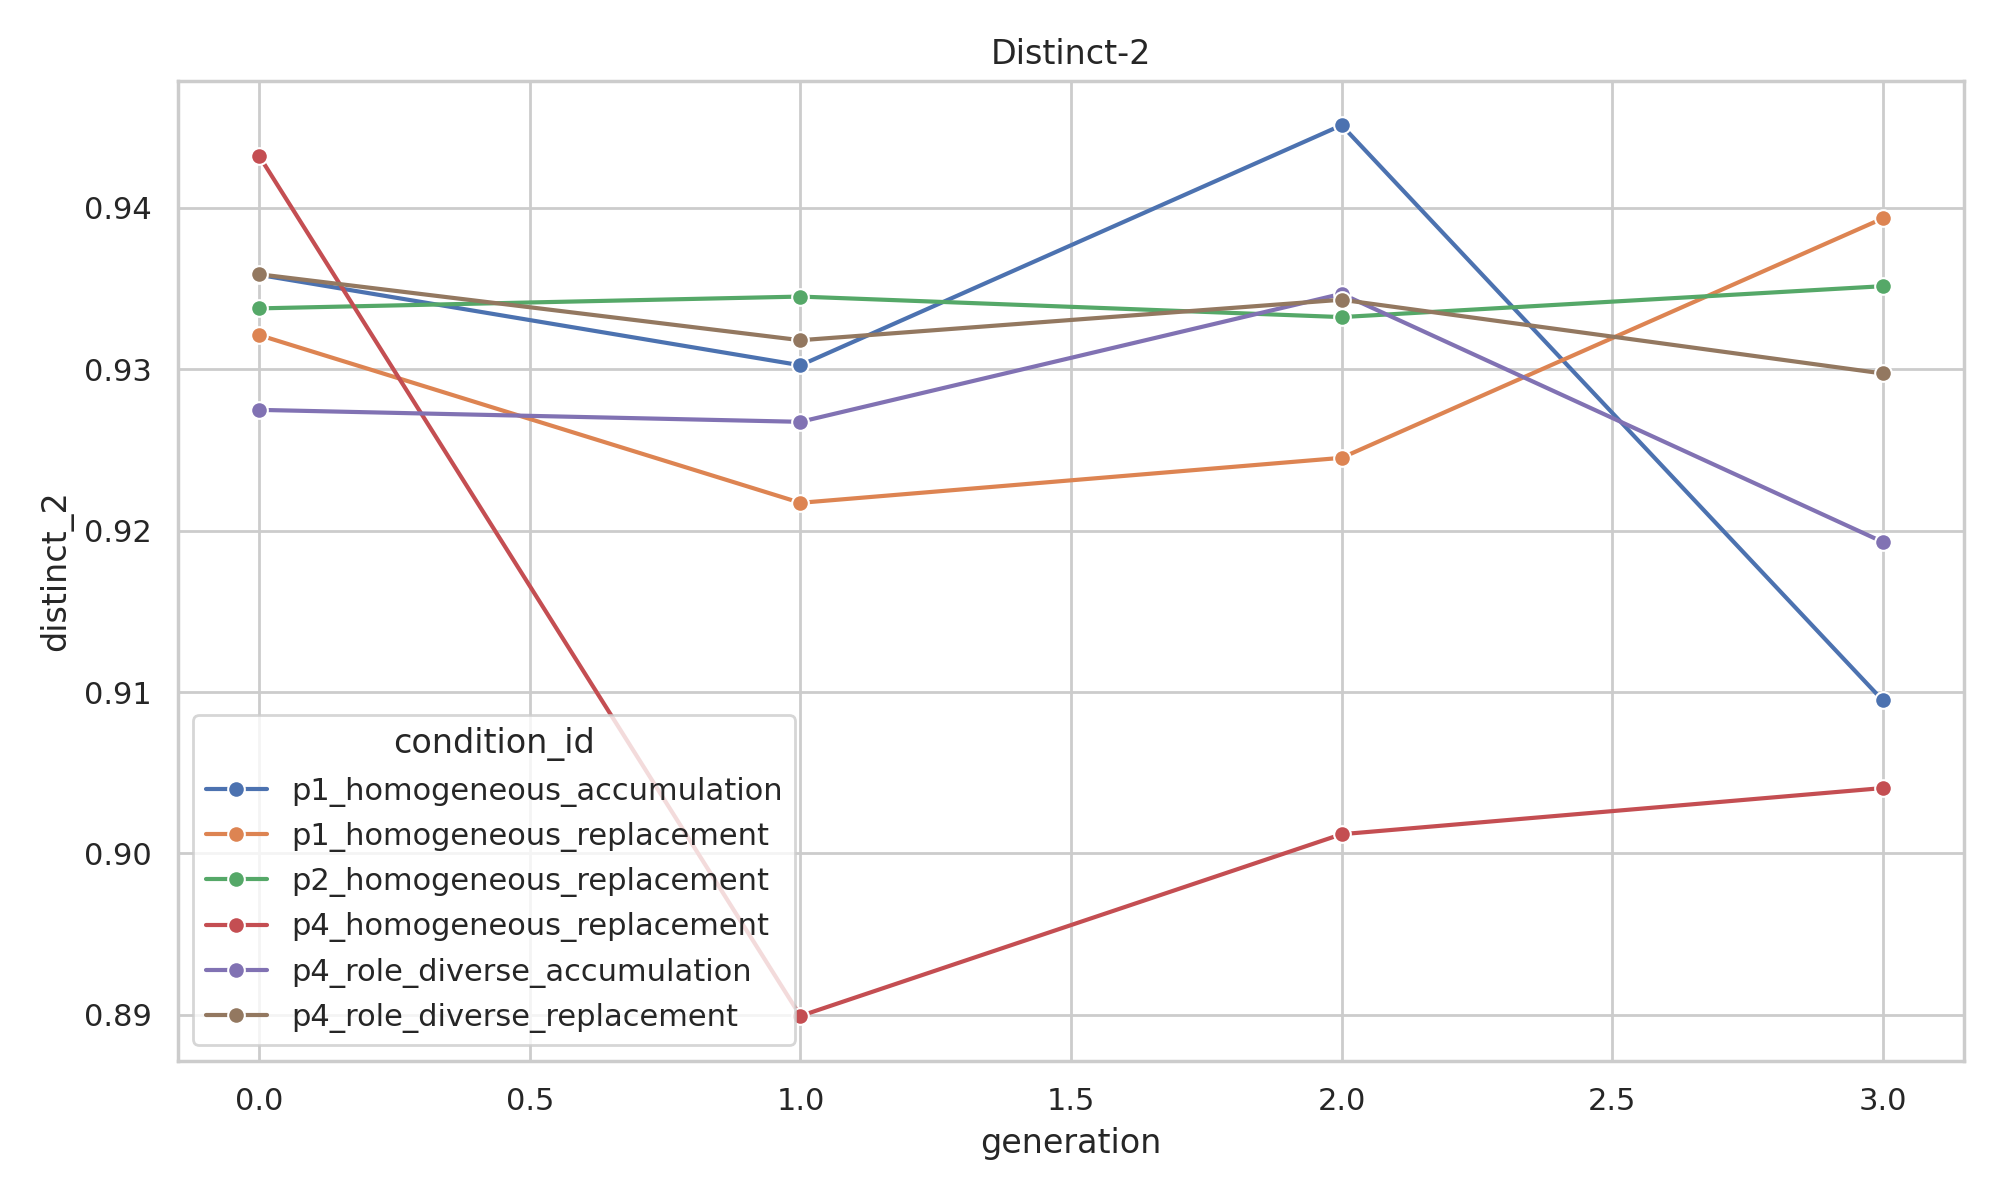
\includegraphics[width=\linewidth]{figures/distinct_2.png}
        \caption{\textbf{Distinct-2.} Lexical diversity changes are condition-specific and do not collapse monotonically.}
    \end{subfigure}\hfill
    \begin{subfigure}[t]{0.24\textwidth}
        \centering
        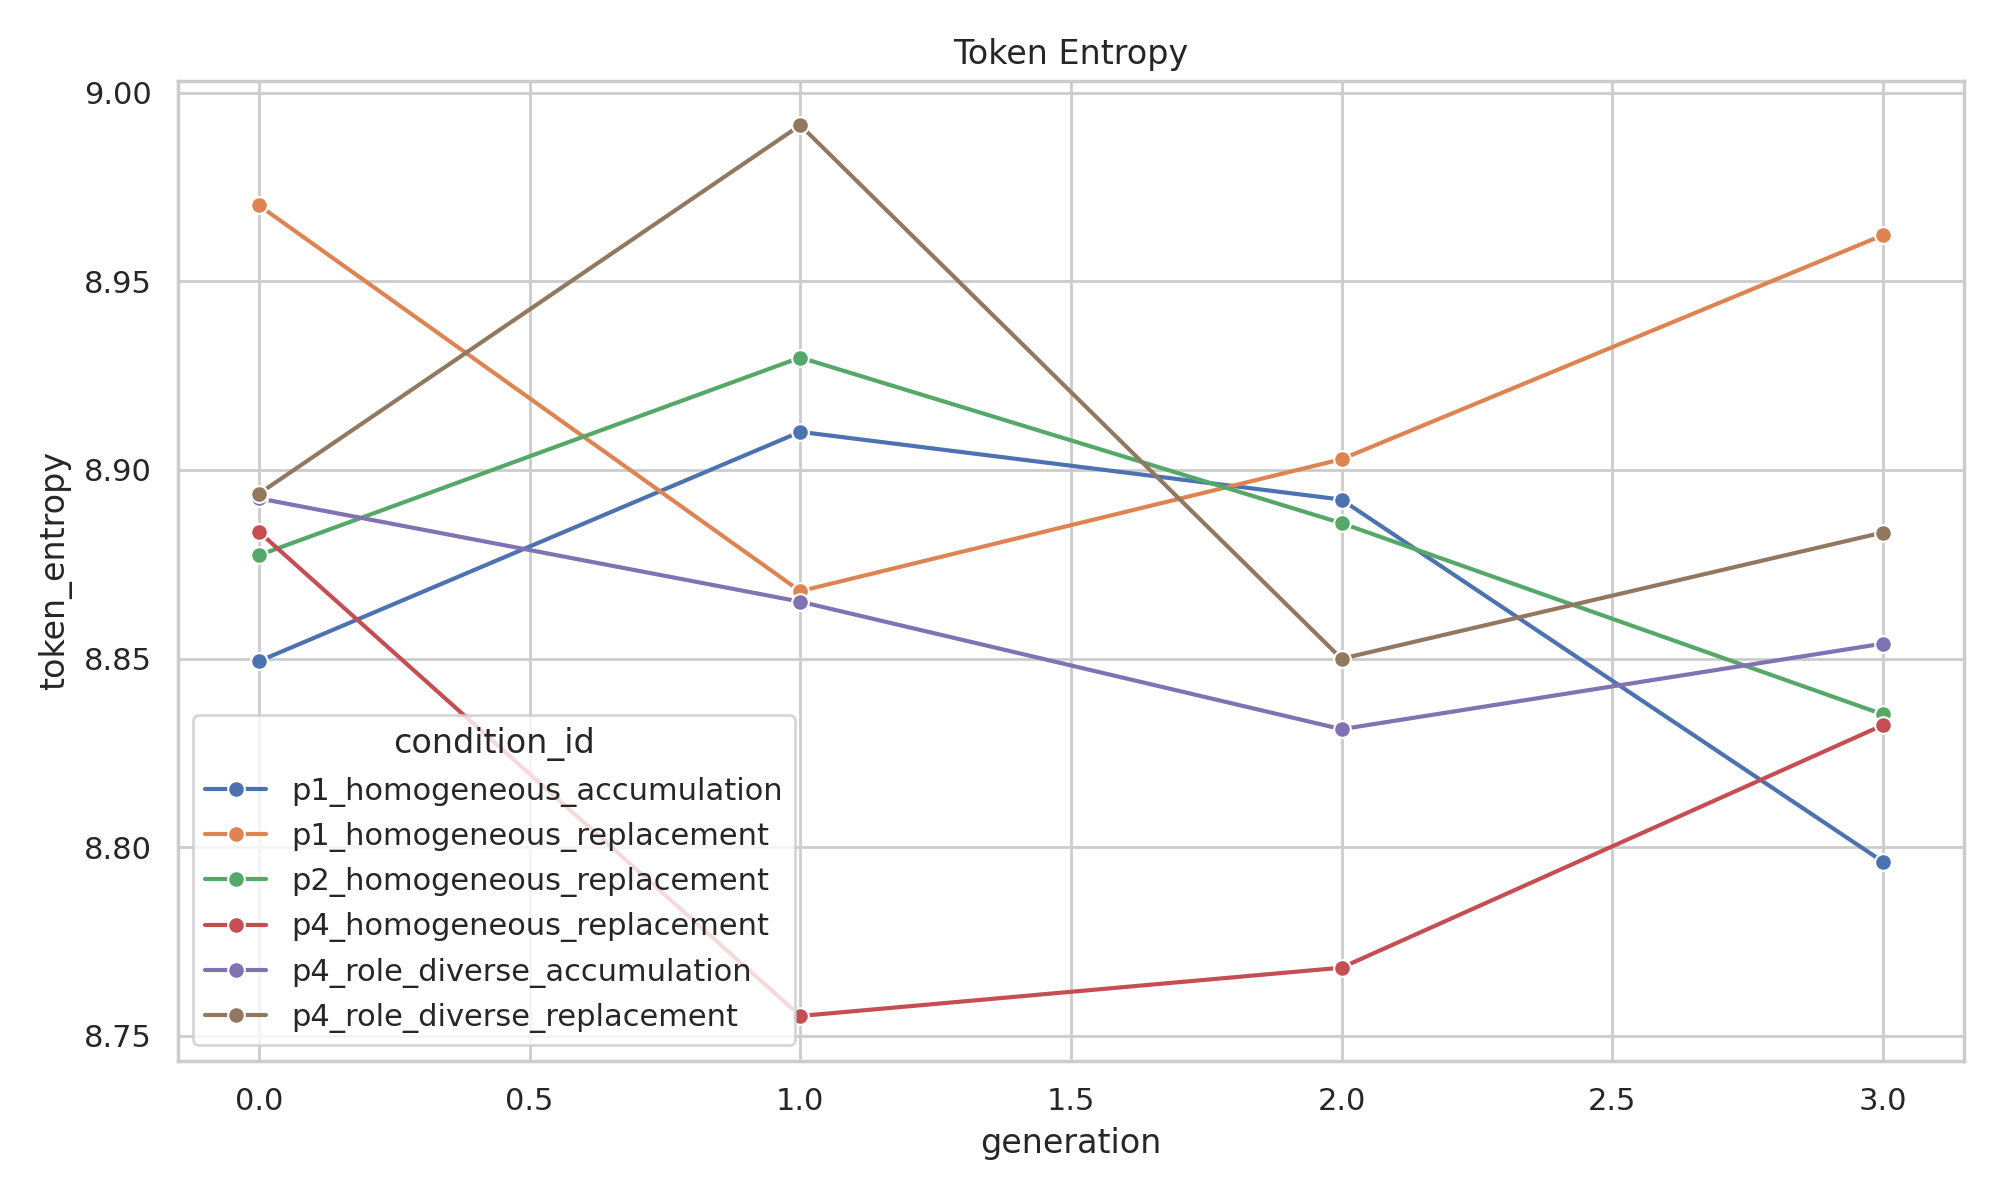
\includegraphics[width=\linewidth]{figures/token_entropy.png}
        \caption{\textbf{Token entropy.} Final entropy remains relatively close across conditions.}
    \end{subfigure}\hfill
    \begin{subfigure}[t]{0.24\textwidth}
        \centering
        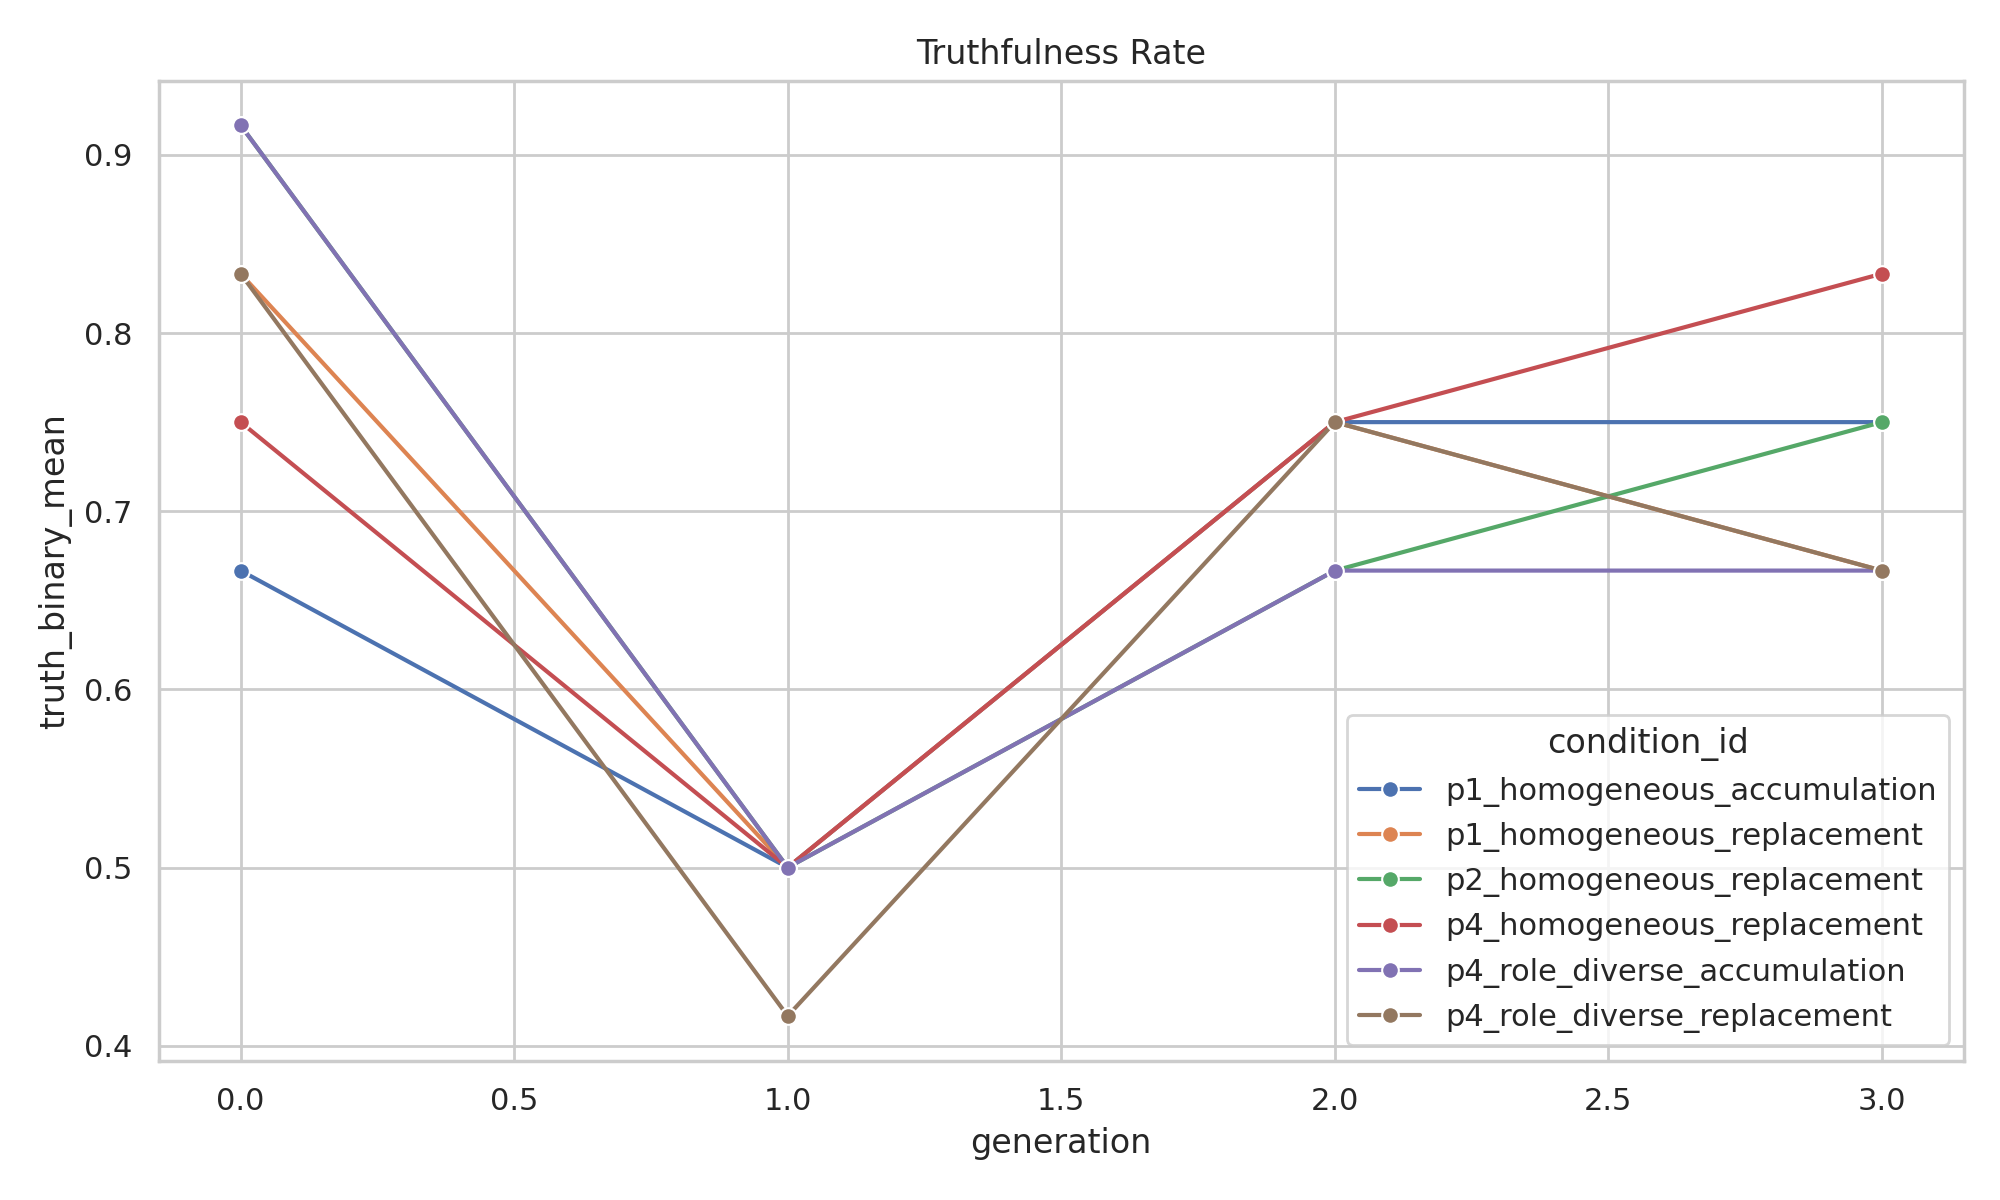
\includegraphics[width=\linewidth]{figures/truth_binary_mean.png}
        \caption{\textbf{Truthfulness.} Every condition suffers a sharp generation-1 drop followed by partial recovery.}
    \end{subfigure}\hfill
    \begin{subfigure}[t]{0.24\textwidth}
        \centering
        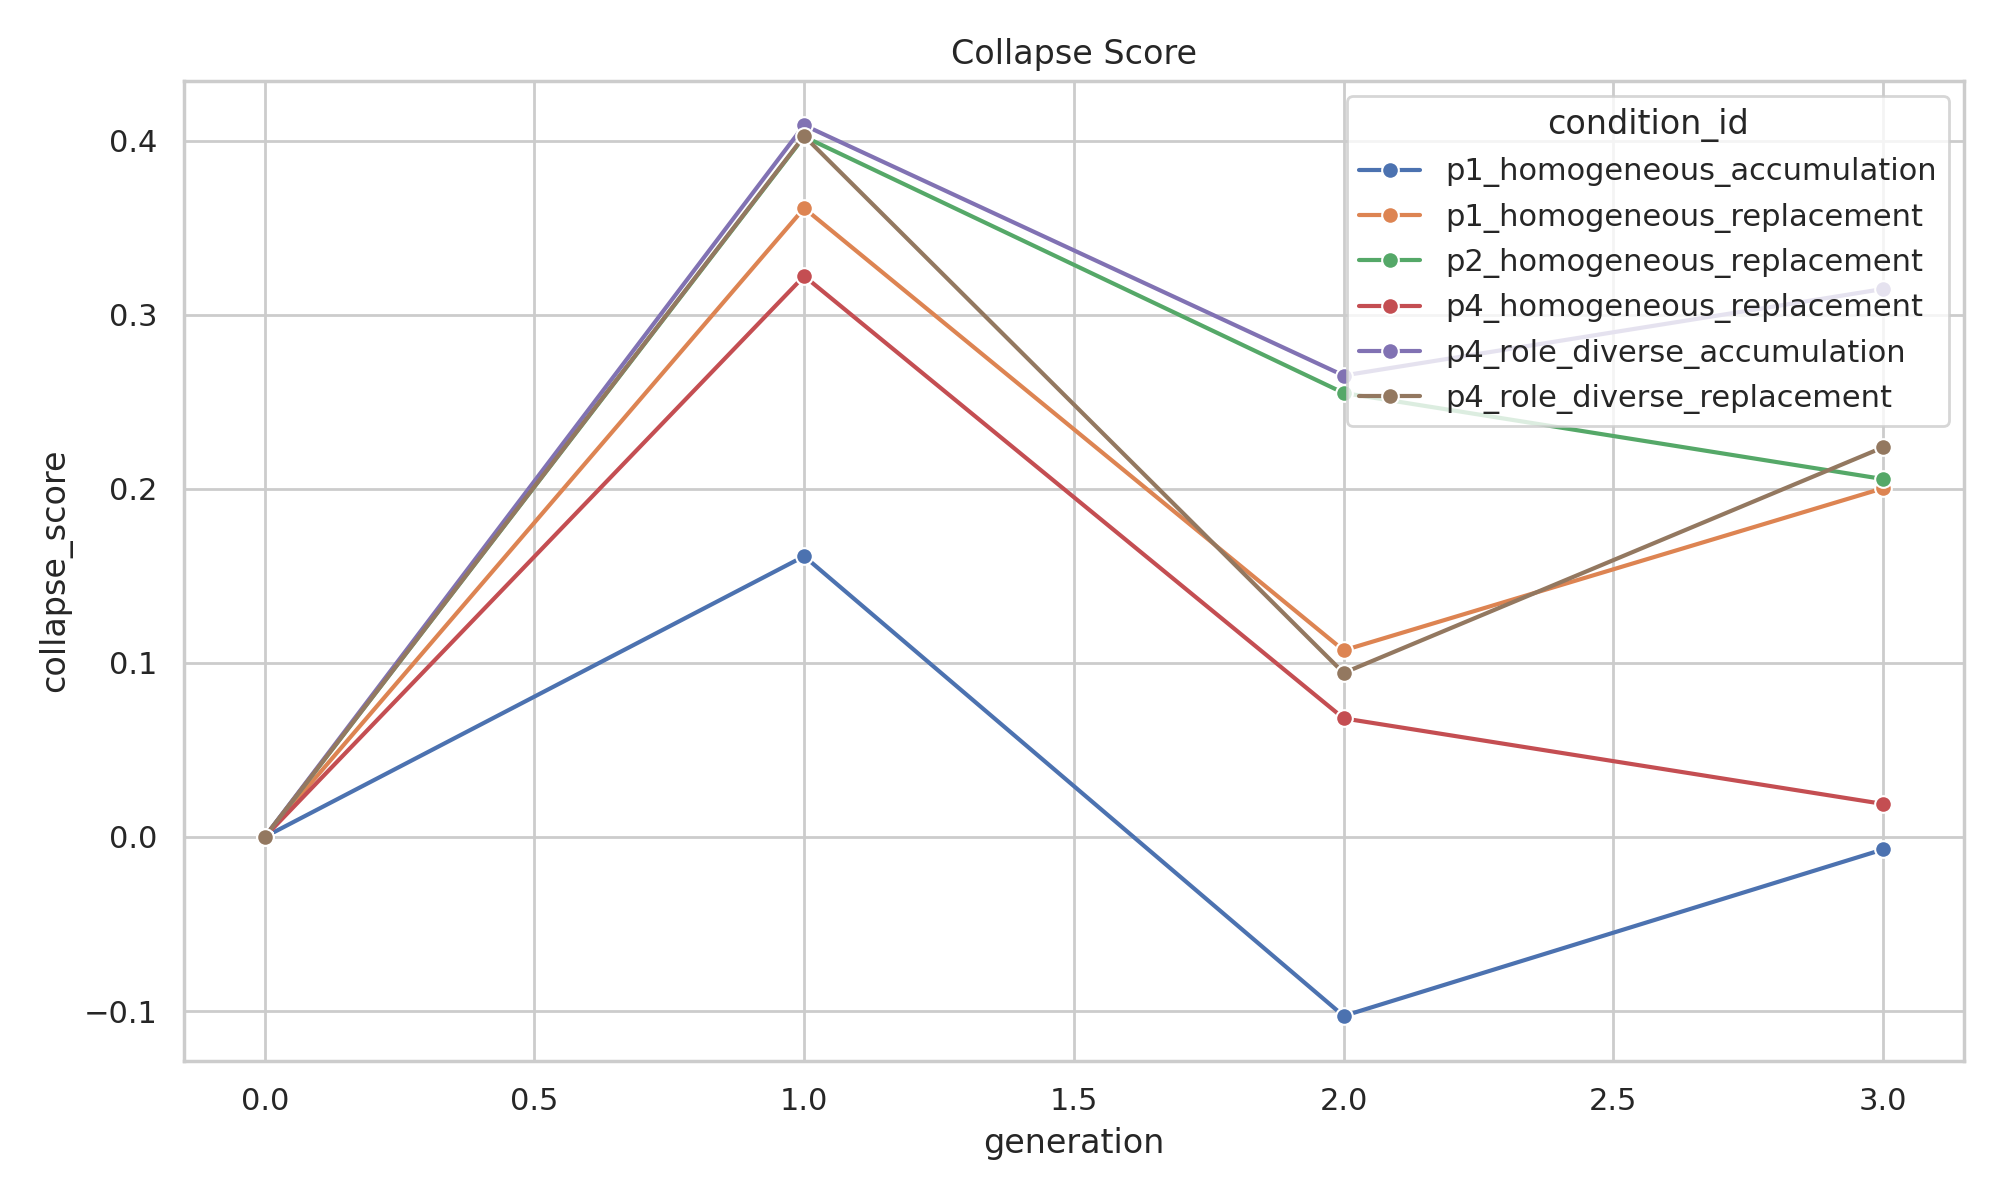
\includegraphics[width=\linewidth]{figures/collapse_score.png}
        \caption{\textbf{Collapse score.} Final rank ordering does not follow nominal population size.}
    \end{subfigure}
    \caption{Trajectory summary across the four tracked generations. The shared qualitative pattern is an early inheritance shock, especially in truthfulness, rather than universal monotonic degradation across all metrics.}
    \label{fig:main-trajectories}
\end{figure*}

\para{Prompt-level role diversity is detectable but not protective.}
The role-diverse conditions have a higher final mean collapse score than the homogeneous conditions: 0.2693 versus 0.1044. They also perform worse than the overall replacement mean in one case and worse than the best homogeneous accumulation condition in both cases. The final-generation Spearman correlation between the individuality proxy and collapse severity is $\rho=0.8281$ with $p=0.0418$. Because higher collapse scores are worse, this association runs opposite the initial hypothesis that more distinct agents would protect the ecosystem.

\para{Accumulation helps modestly on average, but not universally.}
When grouped by data regime, accumulation yields a slightly better mean final collapse score than replacement, 0.1538 versus 0.1622. This direction is consistent with prior accumulation-based anti-collapse findings \cite{gerstgrasser2024model}. However, the effect is not universal in our bounded setup. The best condition uses accumulation, but the worst condition does too. This again suggests that preserving a human anchor matters, but its benefit depends on what kind of diversity and inheritance the system preserves.

\para{Embedding concentration still rises over time.}
Despite partial truthfulness recovery, every condition ends with higher embedding similarity than it started with, which indicates concentration of outputs over time. For example, \textsc{P1-Homogeneous-Accumulation} rises from 0.1579 to 0.2018, \textsc{P4-Homogeneous-Replacement} rises from 0.1580 to 0.2154, and \textsc{P4-Role-Diverse-Replacement} rises from 0.1681 to 0.2179. This matches the broader collapse literature in which diversity can degrade even when top-line utility has not yet failed completely \cite{shumailov2023curse,briesch2023large}.
